%\documentclass[aps,prb]{revtex4}
%\documentclass[aps,prb,twocolumn]{revtex4-1}
\documentclass[showpacs,aps,prb,reprint,superscriptaddress]{revtex4-1}
%\documentclass[showpacs,aps,prl,reprint,superscriptaddress,showkeys,floatfix,citeautoscript]{revtex4-1}
\usepackage{bm}
\usepackage{subfig}
\usepackage{graphicx}
\usepackage{graphics}
\usepackage{amsmath,amssymb,amstext}
\usepackage{amsfonts}

\usepackage{epstopdf}
\usepackage{hyperref}
\usepackage{hyperref}
\hypersetup{
    colorlinks,%
    citecolor=blue,%
    linkcolor=blue,%
    urlcolor=blue
}
%\usepackage{pgf}
\usepackage{tikz}\usetikzlibrary{petri}
%\usepackage{bbold}
%\usepackage{makeidx}
\newcommand{\TS}[1]{{$\rightarrow$ {\sl#1}}}
\newcommand{\LUIS}[1]{\textcolor{blue}{\fbox{Luis} {\sl#1}}}
\newcommand{\Jesus}[1]{\textcolor{red}{\fbox{Jesus} {\sl#1}}}
\begin{document}


\newcommand{\be}   {\begin{equation}}
\newcommand{\ee}   {\end{equation}}
\newcommand{\ba}   {\begin{eqnarray}}
\newcommand{\ea}   {\end{eqnarray}}
\newcommand{\ve}  {\varepsilon}

\newcommand{\nhat}{\hat{n}}
\newcommand{\veck}{\textbf{k}}
\newcommand\ep{\epsilon}
\newcommand\g{\gamma}
\newcommand\s{\sigma}
\newcommand\up{\uparrow}
\newcommand\dw{\downarrow}
\newcommand\down{\downarrow}
\newcommand{\ed}[1]{\ep_{d#1}}
\newcommand{\ket}[1]{\vert #1 \rangle}
\newcommand{\ann}{a^{\dagger}}
\newcommand{\dann}{d^{\dagger}}
\newcommand{\tdots}{t_{dots}}
\newcommand{\gammaA}[1]{\gamma_{A,#1}}
\newcommand{\gammaB}[1]{\gamma_{B,#1}}
\newcommand{\Green}[1]{G_{#1}(\omega) }

\newcommand{\GreenG}[2]{G_{#1}^{ #2} (\omega) }
%\newcommand{\bra}[3]{\langle {#3} \vert}

\newcommand{\super}{\vert \Delta \vert}





%%%%%%%%%%%%%%%%%%%%%%%%%%%%%%%%%%%%%%%%%%%%%%%%%%%%%%%%%%%%%%%%%%%%%%%%%%%%%%%
\title{ Manipulation of Majorana Modes in a Double Quantum Dot }

\author{Jesus D. Cifuentes}
\affiliation{Instituto de F\'{\i}sica, Universidade de S\~{a}o Paulo,
C.P.\ 66318, 05315--970 S\~{a}o Paulo, SP, Brazil}
\author{Luis G.~G.~V. Dias da Silva}
\affiliation{Instituto de F\'{\i}sica, Universidade de S\~{a}o Paulo,
C.P.\ 66318, 05315--970 S\~{a}o Paulo, SP, Brazil}

\date{ \today }

\begin{abstract}

(To be written)


\end{abstract} 
%\pacs{ APS does not use it anymore}
%\keywords{Quantum Spin-Hall effect, Edge transport, Topological insulators}

\maketitle


%%%%%%%%%%%%%%%%%%%%%%%%%%%%%%%%%%%%%%%%%%%%%%%%%%%%%%%%%%%%%%%%%%%%%%%%%%%%%%%
\section{Introduction}
\label{sec:Intro}



In the last few decades the interest in the so called Majorana fermions has been increasing. The particle proposed by the physicist Ettore Majorana  as the real field solution of the Dirac equation describes a fermion which is its own antiparticle, hence it has no charge nor mass. To the date no fundamental particle with these characteristics has been found. However,  theoretical research predicts that Majorana Fermions emerge as quasi-particles at the boundary of certain topological superconductors. \citet{kitaev_unpaired_2001} Recently, the new technological innovations  allowed the observation of Majorana signatures in different topological materials. \citep{mourik_signatures_2012,das_zero-bias_2012,deng_anomalous_2012,zhang_quantized_2018}

Despite the positive experimental results, their is still certain skepticism about the existence of  Majorana Fermions. One of the reasons  is that some properties of Majorana quasiparticles like the expected non-abelian statistics have not been measure. This property is of especial interest due to its promising applications in topological quantum computing. The braiding protocol based on  Majorana's non-abelian statistics is the key to  fault-tolerant quantum computation. \cite{kitaev_fault-tolerant_2003,sarma_majorana_2015} 

% Experimental proposals for braiding measurements have been  proposed  in one dimensional majorana chains.  The system inspired in the famous Kitaev toy model is a promising example of these topological superconductors.  The chain emulates a spinless p-wave superconducting wire. With the adequate combination of magnetic field,  superconducting gap and Rashba spin-orbit coupling  the wire enters into a topological phase in which zero-mode majorana bound states emerge. 

A promising method to detect Majorana modes consists in attaching a quantum dot (QD) to the edges of a Majorana chain in the topological phase and executing transport measurements through the QD. \cite{liu_detecting_2011}  The Majorana mode at the end of the chain then leaks inside the QD \cite{vernek_subtle_2014} which produces a zero-bias conductance peak of half a quanta $\frac{e^{2}}{2h}$ through the dot. This is a Majorana signature which produces half of the expected peak by a regular fermion.  Recently, experiments including hybrid Majorana-QD systems have been performed. \cite{deng_majorana_2016}  In addition, the similarity of this phenomenon with the Kondo effect, where the zero-bias conductance peak takes  $\frac{e^{2}}{h}$, motivated the study of combined Kondo-Majorana physics in this system. \cite{lee_kondo_2013,ruiz-tijerina_interaction_2015} This project revealed the existance of a region of parameters where both, Kondo and Majorana physics, coexist. 

This idea has turned on new lights into the design of quantum architectures, \cite{barkeshli_physical_2015,karzig_scalable_2017}  because today’s precise experimental control over the parameters of QDs - energy levels, tunneling couplings, etc. - offers the unique possibility of manipulating the Majorana modes inside multi-dot systems. The simplest case where Majorana manipulation is possible is in a double quantum dot. So far, no complete analysis of this simple case has been done. The goal of this  project is to fill this gap by realizing a full quantum transport study of the effects of coupling a Majorana mode with a double quantum dot.  By tuning the QD gate voltages and the Majorana couplings we will be able to probe the mobility of the Majoranamodes through the dots. 
 
%  The idea of using hybrid quantum dot-Majoranaheteroestructures to implemtent quantum gates has aquired wide interest in the last years.  One of the insights of these structures is the posibility of manipunaling  Majoranas  in multidot systems by shifting the QD gate voltages and Hence the approach is suitable for the implementation of braiding procedures . The simplest system where Majorana manipulation is possible is  a  double quantum dot (DQD) coupled to a Majoranachain. So far, no complete analysis of this simple case has been done. The goal of this  project is to fill this gap by realizing a full quantum transport study of the effects of coupling a Majorana mode with a double quantum dot.
 
 
  We  considered both interacting and non-interacting cases. For interacting systems we used a obtained the exact transport description . On non-interacting models we used a NRG approach.   We found that in symmetric couplings  In the non-interacting case, we confirmed that shifting the QD’s gate voltage induces the Majorana to tunnel only to the other dot. In addition, an indirect coupling of the second dot could cause destructive interference with the Majorana signature. In the interacticting case,  the NRG simulations confirmed these results and showed that other interacting effects - like Kondo and RKKY \cite{ruderman_indirect_1954,kasuya_theory_1956,yosida_magnetic_1957} - could coexist with the Majorana signatures. On the other hand, when only one QD is coupled to the leads and the other Dot is attached to the QD,  the Kondo effect is annihilated due to the destructive interference  generated by extra dot \cite{dias_da_silva_transmission_2008}. Our study includes how the Majorana mode interacts with these two effects.  
 
 
%  When both dots are coupled to the leads the Double Quantum Dot exhibits an antiferromagnetic interaction known as  Ruderman-Kittel-Kasuya-Yosida (RKKY) interaction. On the other hand, when only one QD is coupled to the leads and the other Dot is attached to the QD,  the Kondo effect is annihilated due to the destructive interference  generated by extra dot \cite{dias_da_silva_transmission_2008}. Our study includes how the Majorana mode interacts with these two effects.  



%  One of the insights of this method is that the information of the qubit is not completely destroyed as in other methods like tunneling spectroscopy. 
%  When Majoranas are connected to multidot systems it is possible to manipulate the Majorana mode inside the QDs  by tuning the gate voltage and  tunnel couplings. This fa

%following the prescription by \citet{oreg_helical_2010} and \citet{lutchyn_majorana_2010}.   

% Despite the positive experimental results, the proof One of the most promising aplications of Majorana Fermions is the implementaition of  braiding procedures  which are the key to implement fault-tolerant quantum computers. 
% Most of the experiments have been based on tunneling spectroscopy in junctions between TS and non metallic (NM) leads, where resonances have been observed at zero energy, consistent with the presence of Majorana zero\textendash energy modes. A downside of the tunneling spectroscopy technique  is that it probes not only the end of the Topological Superconductor(TS), but its bulk as well ,
% which completely destroys the qubit information. A less destroying



% In addition, the use of QDs favors the manipulation of the Majorana mode through the shifting of the dot gate voltage and the hopping parameters.

 
 




% Then the Majorana  as proposed by  \citet{liu_detecting_2011} and consists in coupling a quantum dot (QD) to the end of a TS. The analysis performed by Liu of this model revealed a  when the TS is in the topological phase,  which a signature of
% Majorana physics. On 2014, \citet{vernek_subtle_2014} showed that the Majorana Bound State at the end of the TS actually leaks inside the QD , which produces the conductance decay. and the model has been based for braiding experimental proposals.










% To the date experimental procedures have been put forward. ery recently the first evidence of Majorana end states
% in TS has been found in multiple experiments


% as quasi-particles in certain types of topological materials have increased. The Majoranas are fermions that are their own anti-particle, hence have no charge nor mass. 
% The Majorana is predicted to be one of the most suitable alternatives to implement fault-tolerant quantum computers. Many experiments showing Majorana signatures in the conductivity have been performed. 





% Basics of Majorana Bound states:  zero-energy edge states in 1D topological superconductors.  

% Discovery on semiconductor nanowires \cite{Oreg:Phys.Rev.Lett.:177002:2010,Lutchyn:Phys.Rev.Lett.:77001:2010,Alicea:Reports:2012} etc. Experimental results \cite{Mourik:Science:1003:2012} \LUIS{Add others.}


% Leaking of Majorana to a QD: \cite{vernek_subtle_2014}, Interplay of Kondo and Majorana\cite{ruiz-tijerina_interaction_2015} Important results: Majorana and Kondo co-exist in the quantum dot even if the dot is non-topological.

% More recent experimental results: Deng et al. \cite{deng_majorana_2016} attached a QD to the end of a nanowire.

% Here we study the coupling of a MBS to a \emph{double} quantum dot system. 

% \TS{Punchline} Multidot systems offer the possiblity of ``moving'' Majoranas aroung using gate voltages and couplings. ossibility of Majorana braiding. Here, we study the simplest case, which is a double dot system.

%%%%%%%%%%%%%%%%%%%%%%%%%%%%%%%%%%%%%%%%%%%%%%%%%%%%%%%%%%%%%%%%%%%%%%%%%%%%%%%
\section{Model and methods}
\label{sec:modelmethods}

%\LUIS{Jesus, put the description of the system and the Hamiltonian here. Put a schematic figure of the DQD setup as well}




We consider the setup shown in Figure \ref{fig:GenModel} in which a Majorana Bound State (MBS) at the edge of Topological Superconductor(TS) is coupled to a double quantum dot (DQD), which is attached to a single metallic lead. The Hamiltonian of this system can be partitioned in four terms: the DQD Hamiltonian $H_{DQD}$ , the Lead Hamiltonian $H_{Lead}$ , the DQD-lead interaction  $H_{DQD-Lead}$ and the coupling between the DQD and the Majorana mode $H_{M-DQDs}$ and   
\begin{equation}
H=H_{DQD}+H_{Lead}+H_{DQD-Lead}+H_{M-DQD} 
\label{eq:Model}
\end{equation}


%-----------F I G U R E  1 ------
\begin{figure}[bt]
\begin{center}
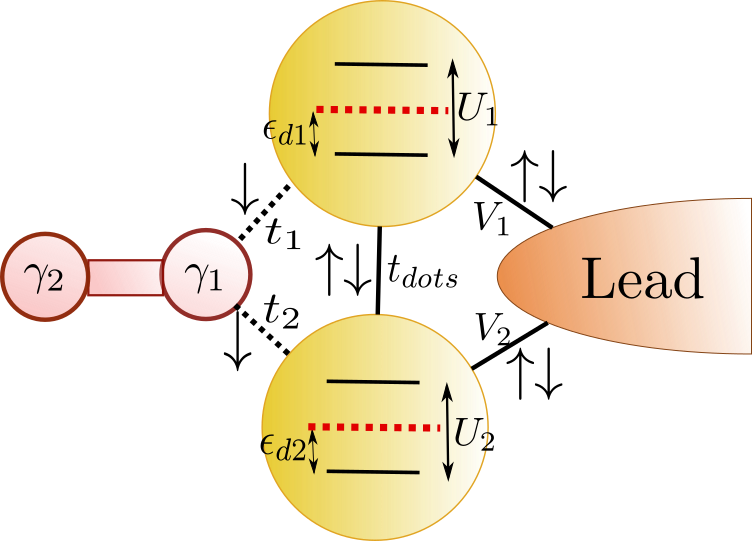
\includegraphics[scale=0.4]{Graficos/GenModel.png}
\caption{ DQD-Majorana set-up. Solid lines: standard coupling. Dashed lines: Majorana spin-$\dw$ effective couplings \eqref{eq:H_MDQD}. The atomic energy levels appear inside each QD. Red dashed horizontal lines represent the Fermi level.  
}
%
\label{fig:GenModel}
\end{center}
\end{figure}
%-----------E N D  F I G U R E  1 ------


%-----------F I G U R E  1 ------
% \begin{figure}[bt]
% \begin{center}
%     \subfloat[\label{fig:GenModel}]{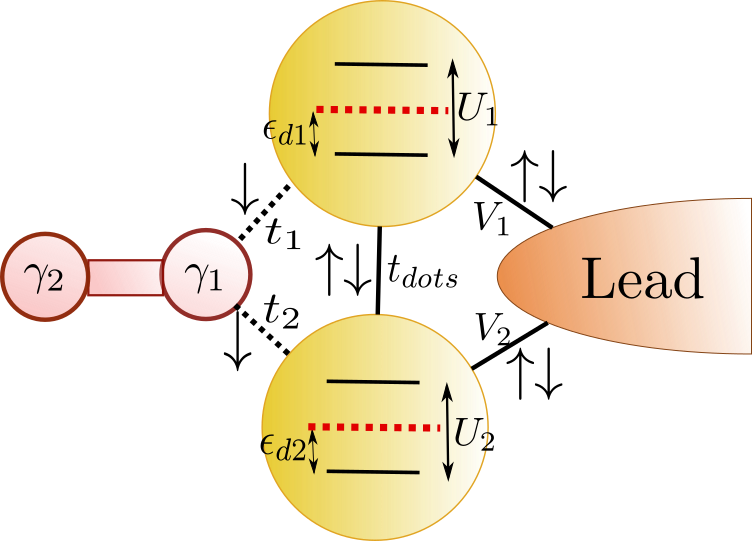
\includegraphics[scale=0.25]{Graficos/GenModel.png}} \hspace{2mm}
%      \subfloat[\label{fig:transport}]{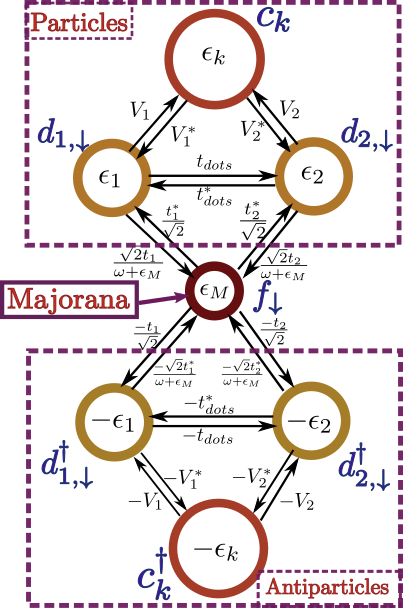
\includegraphics[scale=0.25]{Graficos/GraphM-DQD.png}} 
% \caption{ 
% }
%

% \end{center}
% \end{figure}
%-----------E N D  F I G U R E  1 ------




The interacting Anderson Model describes the DQD-lead system  
%d_{i\sigma}^{\dagger}d_{i\sigma}
\begin{align}
\begin{split}
    H_{DQD}=&  \sum_{i\in\{1,2\}} \sum_{\sigma\in \{ \dw , \up\}}  \left(\epsilon_{di}+\frac{U_i}{2}\right)\hat{n}_{i\sigma}+ \frac{U_i}{2}(\sum_{\sigma} \hat{n}_{i\sigma}-1)^{2} \\ 
&\ \ \ \ \ + \sum_{\sigma \in \{\up , \dw\}} \tdots(\dann_{1\sigma}  d_{2\sigma}+\dann_{2\sigma}  d_{1\sigma}), \label{eq:H_DQD}
\end{split}
\end{align}

and 
\begin{eqnarray}
H_{Lead} & = & \sum_{\mathbf{k}\sigma }\epsilon_{\mathbf{k}}c_{\mathbf{k}\sigma }^{\dagger}c_{\mathbf{k}\sigma } \label{eq:H_L}\\ 
H_{DQD-Lead} & = &  \sum_{\mathbf{k}\sigma }\sum_{i\in\{1,2\}}V_{i\textbf{k}} c_{\mathbf{k}\sigma }^{\dagger}d_{i\sigma}+V^*_{i\textbf{k}} d_{i\sigma}^{\dagger}c_{\mathbf{k}\sigma }  \label{eq:H_DQDL},
\end{eqnarray}
%
where $\ed{i}$ is the energy level of dot $i$, $U_i$ is the Coulomb repulsion and $\tdots$ is the coupling parameter between both QDs. The operator $\dann_{i\sigma}$ creates a particle in dot $i$ with spin $\sigma$ and $\hat{n}_{i\sigma}:=d_{i\sigma}^{\dagger}d_{i\sigma}$ is the particle number operator of state $i$.  $c_{\mathbf{k}\sigma }^{\dagger}$ is the creation operator a particle with momentum $\mathbf{k}$ and spin
$\sigma$ in the lead.  $\epsilon_{\mathbf{k}l}$ is the corresponding energy
 and $V_i(\textbf{k})$ describes the tunneling coupling between the lead and dot $i$ . \\

% To model the interaction between the DQD and the Majorana Mode we define the Majorana operators as the

The Majorana modes are modeled as a superposition of the creation and annihilation operators of a spin $\dw$ particle $f_\dw$
\begin{equation}
    \gamma_1 := \frac{1}{\sqrt{2}} \left( f^\dagger_{\dw} + f_{\dw}\ \right) , \gamma_2 := \frac{i}{\sqrt{2}} \left( f^\dagger_{\dw} - f_{\dw} \right). \label{eq:MajOp}
\end{equation}


This makes possible to define an effective coupling between the Majorana Mode and the DQD by attaching $\gamma_1$ with the spin-$\dw$ channel in the QDs

%H_{TS} & = & 2\epsilon_{m}\gamma_{1}\gamma_{2}\nonumber \\
\begin{eqnarray}
H_{M-DQD} & = &  \sum_{i=1}^2t_{i} \left(d_{i\downarrow}^{\dagger}\gamma_{1}+\gamma_{1}d_{i\downarrow}\right) + \epsilon_M \gamma_1\gamma_2. 
% \\
% & = &  \sum_{i}t_{i} \left(d_{i\downarrow}^{\dagger}f^\dagger_{\dw} + 
% f_{\downarrow}d_{i\dw} +d_{i\downarrow}^{\dagger}f_{\dw}+
% +f_{\downarrow}^{\dagger} d_{i\downarrow}\right).
\label{eq:H_MDQD}
\end{eqnarray}
where $t_i$ is the coupling parameter between the Majorana mode and QD $i$. $\epsilon_m$ is the coupling energy between both Majorana modes. This effective model is able to reproduce the physical effects of more elaborated couplings \cite{ruiz-tijerina_interaction_2015} such 

\citeauthor{ruiz-tijerina_interaction_2015}  showed that this effective coupling  is able to reproduce effectively the transport effects of  the Kitaev chain in the topological phase is attached to a single QD.  \\




% \begin{equation}
%     \omega\Green{A,B}&=\delta_{A^{\dagger},B}+\Green{\left[A,H\right],B}
% \end{equation}

% \Jesus{Should I put the other terms? }



 
% ---------------------------------------------------
% \newpage
\subsection{Methods}

\subsection{Non-interacting case \label{sec:non-interactingMethods}}

To study the non-interacting case $(U=0)$, we use Zubarev's ballistic transport approach \cite{zubarev_double-time_1960} to compute the Green functions associated to both quantum dot operators $(\Green{d_1d^\dagger_1},\Green{d_2d^\dagger_2})$. The detailed procedure is included in Appendix \ref{sec:Appendix_alg}. The transport equations define a linear system where the Hamiltonian parameters $(t_1,t_2,\epsilon_1 \ldots)$ and the energy $\omega$ are taken as fix variables. The flow graph in FIG.\ref{fig:Transport} depicts the linear map associated to the transport in an hybrid Majorana-DQD system (see \eqref{eq:TransportMatrix} ). The energies of each operator are located at the center of the vertexes while the vertex couplings represent the off-diagonal terms.  The Majorana mode connects two regions of the graph, both of them representing a DQD. The upper DQD is conformed by annihilation operators while the lower one is formed by creation operators. The couplings in the lower part are the  upper parameters multiplied by $-1$. 

To simplify the solution of this system we used a graph linear algorithm  that speeds-up the process of Gauss-Jordan elimination. \cite{spielman_algorithms_2010}. Starting with the flow graph at FIG.\ref{fig:Transport} (a), the algorithm successively "pops"  the vertexes till only one vertex remains in the the graph. Popping a vertex must be understood as the Gaussian elimination of the line and the column in the transport matrix containing that vertex (see Section \ref{sec:Appendix_alg}). This modifies the energies of the vertexes and the coupling parameters. Changing the order of elimination of the vertexes could lead to different equivalent representations of the final polynomial. Finding a suitable elimination order could significantly reduce the complexity of the solution \cite{spielman_algorithms_2010}.  


This graph-linear solver algorithm turns out to be particularly good for Majorana systems  since the Majorana fermion is a natural cutting point that divides the graph in two sections. This allows us to exploit the graph structure to simplify the solution of the system  by selecting a suitable order of vertex-elimination . Fig.\ref{fig:Transport} depicts this process. In the first step (a) to (b), we pop consecutively the vertexes $c_{k,\dw},c_{k,\dw}^\dagger , d_{2,\dw} , d^\dagger_{2,\dw}$. The new parameters $\epsilon^{\pm}_{DQD}$ , $M_2$ and $T_\pm$ (See \eqref{sec:Appendix_alg}) are functions of $\epsilon_1 , \epsilon_2 , t_1,t_2$, etc . These functions gather the transport information  through the popped vertexes . The next step is to pop vertexes $d_{1,\dw}^\dagger$ and $f_{\dw}$, which condensed the transport information of the whole system into the remaining vertex $d_{1,\dw}$ . As shown in section \ref{sec:Appendix_alg} the energy of vertex $d_{1,\dw}$ is $\omega - \Green{d_1\dw d^\dagger_1\dw } $, hence giving a very compact expression for the Green function

% This process can be observed graphically in figure \ref{fig:Transport}. In the first step (a) to (b), we pop-out consecutively the vertexes $c_{k,\dw},c_{k,\dw}^\dagger , d_{2,\dw} , d^\dagger_{2,\dw}$. The transport information through these vertexes is   in the operators  $d_{1,\dw}$, $d_{1,\dw}^\dagger$ and $f_\dw$, such that the energies $\epsilon^{\pm}_{DQD}$ accumulate the information of both double quantum dots while the couplings are modified to $T_\pm$. The last step is to pop-out vertexes $d_{1,\dw}^\dagger$ and $f_{\dw}$. At the end of the whole process the energy of the remaining vertex $d_{1,\dw}$ contains the green function $\Green{d_1\dw d^\dagger_1\dw } $ giving this very compact expression
\begin{equation}
    G_{{d_{1\downarrow},d_{1\downarrow}^{\dagger}}}\left(\omega\right)=\frac{1}{\omega-\epsilon_{DQD}^{+}-\frac{\left\Vert T_{+}\right\Vert ^{2}}{\omega-\epsilon_{M2}-\frac{\left\Vert T_{-}\right\Vert ^{2}}{\epsilon_{DQD}^{-}}}}.
    \label{eq:Green_NonInteracting}
\end{equation}


% Note also that the spin-$\up$ green functions  can be obtained by replacing the Majorana couplings $t_1,t_2 = 0$.
The final result will depend on the broadening parameter of QD $i$ with the lead $(\Gamma_i)$. This broadening satisfies the equation

\begin{equation}
   -i\Gamma_i = \lim_{s\rightarrow 0} \sum_{\boldsymbol{k}}\frac{V_{i}^{*}V_{i}}{\omega+ is -\epsilon_{\boldsymbol{k}}}.
\end{equation}

By convention we will take $\Gamma_1$ as the energy unit for the rest of the project. Finally we compute the DOS 


\begin{equation}
    \rho_{1\sigma}(\omega)=-\frac{1}{\pi} \textrm{Im} \left[G_{d_{1\sigma},d_{1\sigma}^\dagger}(\omega))\right].
    \label{eq:Density of States}
\end{equation}
Similar results can be obtain for the DOS of the second $\rho_{2\sigma}$ . Comparing these results for both dots at the Fermi energy we will be able to determine which dot exhibits a Majorana signature.


% The green functions $(\Green{d_1d^\dagger_1},\Green{d_2d^\dagger_2})$  obtained through Gauss-Jordan elimination constitute fractional polynomial with more than $300$ independent linear components. To provide a tractable decomposition of this polynomial we used a graph theory-inspired linear algorithm that emulates a Laplacian linear solver . Although this Hamiltonian is not Laplacian,  this method still provides a shortcut to Gauss-Jordan elimination by taking advantage of the minimal cuttings in the graph. As a matter of fact , this graph approach is especially good for Majorana systems  since the Majorana fermion is a natural cutting point that divides two sections of the graph.  
% In addition the graph contraction facilitates a legible representation of the fractional polynomial.
% The solution of this problem can be achieved through 
% In a system without Majorana fermions these two regions are disconnected. The new physical   

% The process of Gauss-Jordan elimination used to solved this cases can be strongly speede

% The solution for the green function  will finally be a polynomial fraction over these variables. 

% This can be done by  Gauss-Jordan elimination, noting that after each elimination process we need to carry on the account in terms of these variables.   When the number of operators in the Hamiltonian increases the number of terms in the polynomial grows-up exponentially. This reveals the importance of exploring new methods that could simplify the solution.   \\



%-----------F I G U R E  2 ------

    \begin{figure}[t]
    \begin{center}
    \centering
     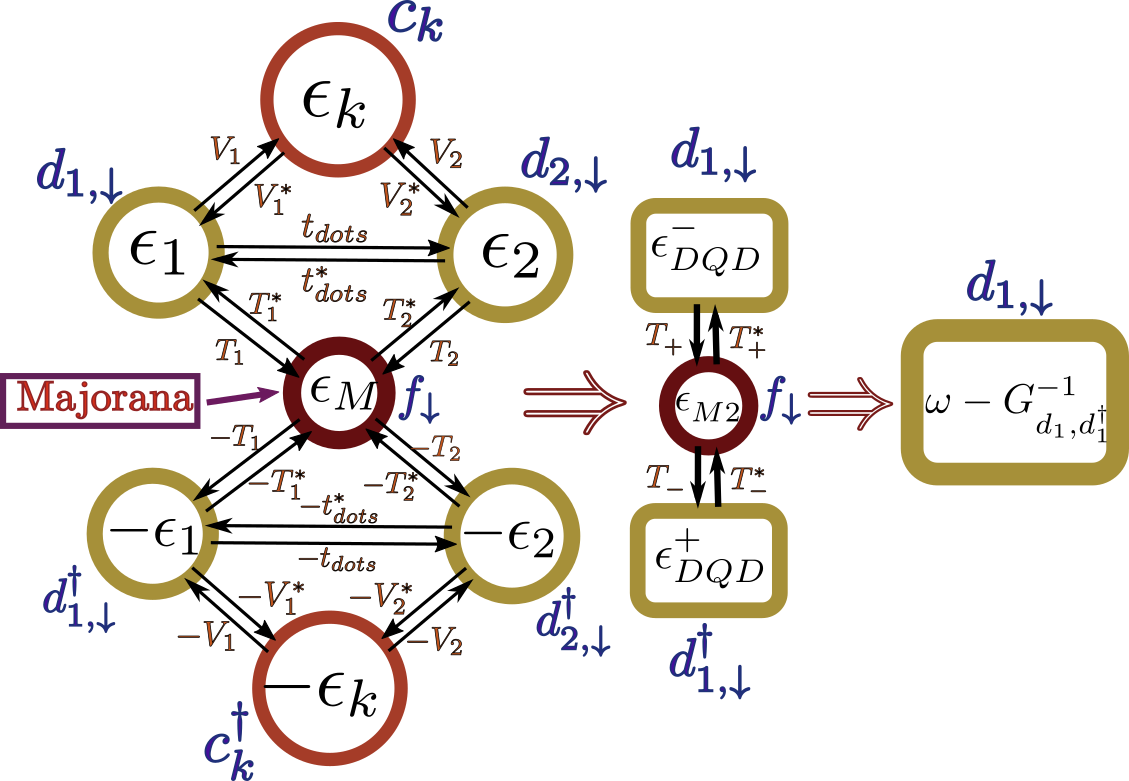
\includegraphics[scale=0.29]{Graficos/Graphs-DQD-M-Pro.png}
    % 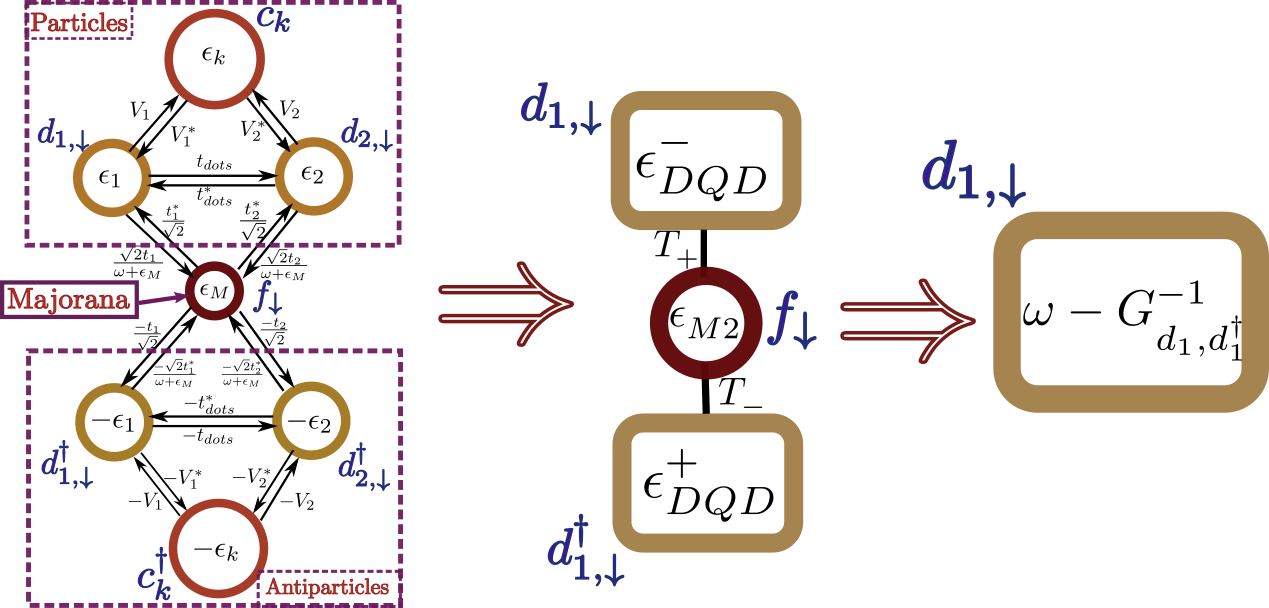
\includegraphics[scale=0.25]{Graficos/graphContractions.png}
    \caption{ Transport flow in a DQD Majorana system.   \label{fig:Transport}
    }
    %
    
    \end{center}
    \end{figure}

%-----------E N D  F I G U R E  2 ------

%

\subsection{Interacting case (NRG)}
For the interacting case, we used the Numerical Renormalization Group (NRG) approach \cite{wilson_renormalization_1975,sindel_numerical_2005,bulla_numerical_2008}. The algorithm assumes a coulomb repulsion of $U =17.3\Gamma_1$ at both dots and a cut-off energy $D=2U=34.6\Gamma_1$. The spacing between the nearest energy levels is assumed to be higher than $D$, hence only one level is relevant in dynamics of the system. Particle-Hole-Symmetry at each dot is obtained when  $\epsilon_i = \frac{U}{2}$. At this point, there is an odd number of electrons at each dot. Hence, at sufficiently low temperature the system will exhibit the characteristic Kondo peak \citet{wilson_renormalization_1975}. Observing how the Kondo-effect interacts with the Majorana signature in the double quantum dot is also an insight of this project. 


To  improve the efficiency of the code we took advantage of the preserved symmetries: The spin-$\up$ particle number $\hat{N}_\up$ and the spin-$\dw$ parity $\hat{P}_\dw = \pm $ ($+$ even, $-$ odd). The spin-$\dw$ particle number is not preserved due to the majorana coupling \ref{eq:H_MDQD} . The initial Hamiltonian organized in blocks according to these symmetries. This structure is preserved during the entire process. The spectral functions are then computed through the Density Matrix Renormalization Group (DM-NRG) approach \cite{hofstetter_generalized_2000}.
  
%   To unify the units of the interacting and non-interacting case we pick $U=8.69\Gamma_1$ and we let $D = 2U_1=17.3 \Gamma_1$.
 \section{Results}
 
     \subsection{Non-interacting dots}
     In non-interacting dots $(U=0)$, the density of states at each dot can be obtained from equation \eqref{eq:Density of States} by replacing the green function at \ref{eq:Green_NonInteracting}. The manipulation of the Majorana mode is achieved by  tuning the model parameters $(t_1,t_2, \epsilon_1 , \epsilon_2 , t_dots)$. Two types of majorana signatures are observed. 
     
     \begin{itemize}
         \item \textbf{Type I: }  The spin-$\dw$ DOS is the half of the spin-$\up$ DOS  at the Fermi energy $(\rho_\dw(0)=\rho_\up(0))$. 
         \item \textbf{Type II: } The spin-$\dw$ Fermi energy is equal about $5.2$. This is the value such that  $\pi  \Gamma_1 \rho_\dw(0) = 0.5$, characteristic of a decay of half a quanta in the conductivity. 
     \end{itemize}
     
     
     
     
     

 
 
 %-----------F I G U R E  3 ------
\begin{figure}[bt]
\begin{center}
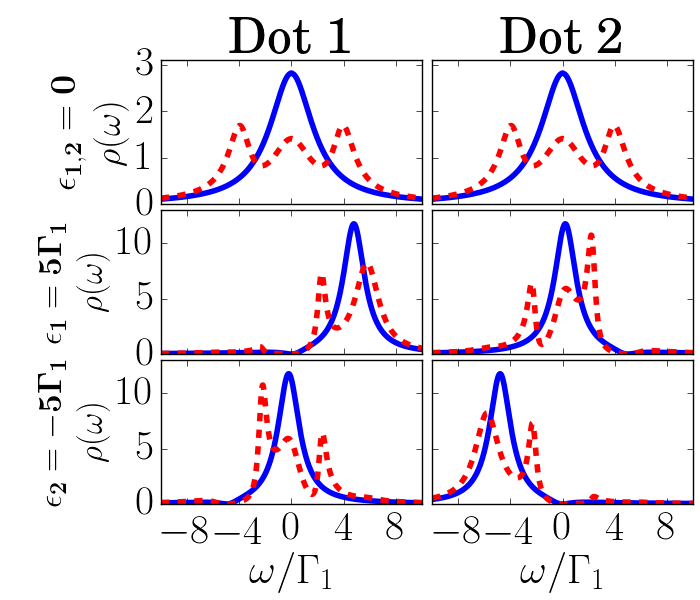
\includegraphics[scale=0.48]{Graficos/t1=t2.png}
\caption{ DQD-Majorana set-up. Solid lines: standard coupling. Dashed lines: Majorana spin-$\dw$ effective couplings \eqref{eq:H_MDQD}. The atomic energy levels appear inside each QD. Red dashed horizontal lines represent the Fermi level.  
}
%
\label{fig:GenModel}
\end{center}
\end{figure}
%-----------E N D  F I G U R E  3 ------

 %-----------F I G U R E  4 ------
\begin{figure}[bt]
\begin{center}
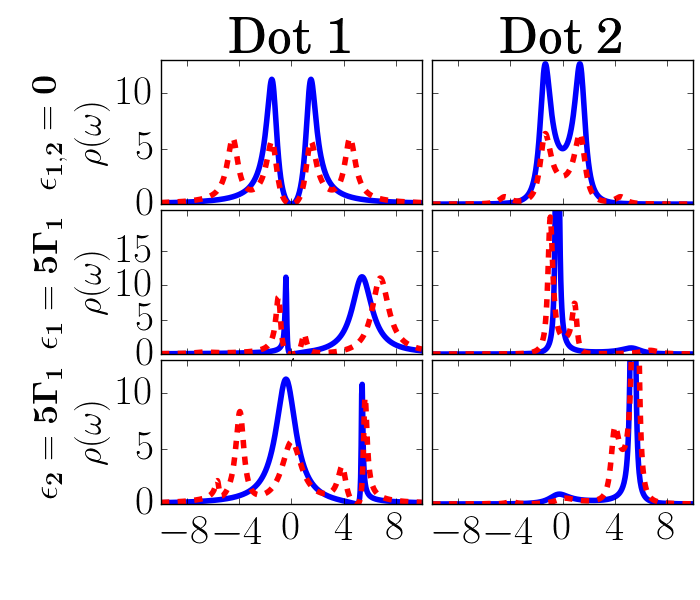
\includegraphics[scale=0.48]{Graficos/t2=0.png}
\caption{ DQD-Majorana set-up. Solid lines: standard coupling. Dashed lines: Majorana spin-$\dw$ effective couplings \eqref{eq:H_MDQD}. The atomic energy levels appear inside each QD. Red dashed horizontal lines represent the Fermi level.  
}
%
\label{fig:GenModel}
\end{center}
\end{figure}
%-----------E N D  F I G U R E  4 ------


 %-----------F I G U R E  5 ------
\begin{figure}[bt]
\begin{center}
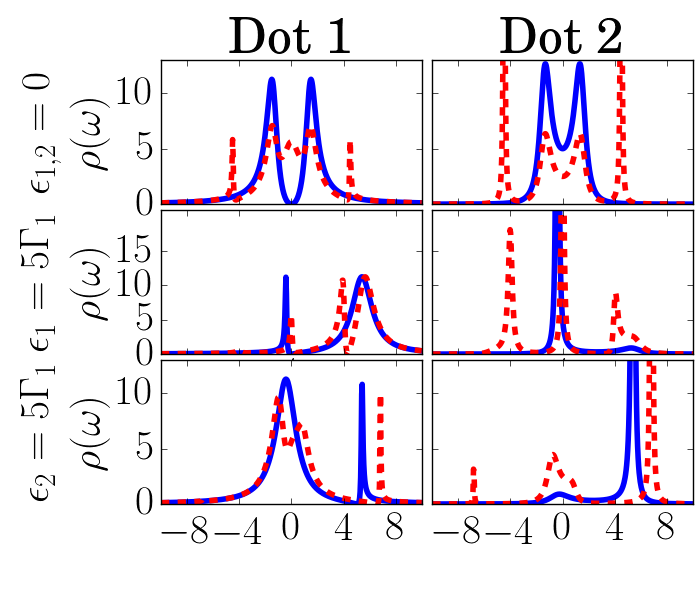
\includegraphics[scale=0.48]{Graficos/t1=0.png}
\caption{ DQD-Majorana set-up. Solid lines: standard coupling. Dashed lines: Majorana spin-$\dw$ effective couplings \eqref{eq:H_MDQD}. The atomic energy levels appear inside each QD. Red dashed horizontal lines represent the Fermi level.  
}
%
\label{fig:GenModel}
\end{center}
\end{figure}
%-----------E N D  F I G U R E  5 ------
 
 
 \subsection{Manipulation in non-interacting QDs}
 \subsection{Manipulation in interacting QDs}
 
 
 
%  spin-$\dw$ particle number $\hat{N_\dw}$ is not preserved due to the term $(d_{i\downarrow}^{\dagger}f^\dagger_{\dw} + 
% f_{\downarrow}d_{i\dw})$ in $H_{M-DQD}$ at \eqref{eq:Majorana-ham}. However the  spin-$\up$ particle number $\hat{N}_\up$ and the parity of spin-$\dw$ particles $\hat{P}_\dw = \pm $ ($+$ even, $-$ odd) are still conserved. \\

 %For convenience we use $D$ as energy unit.  \\






%---------------------------------------------------------------------------





    
\section{Concluding remarks}
\label{sec:Conclusions}

Conclusion goes here.

\begin{acknowledgments}
The authors thank Edson Vernek for enlightening discussions.  L.G.G.V.D.S. acknowledges financial support by CNPq (grants No. 307107/2013-2 and 449148/2014-9), and FAPESP (grant No. 2016/18495-4).
\end{acknowledgments}

% \LUIS{Only ONE bib file}

%---------------------- Apendix A------------------------


%-----------------------------------------------------------

%\bibliographystyle{unsrtnat}
%\addcontentsline{toc}{section}{\textbf{References}}
\bibliography{Majorana_DQD}

 \appendix

 
 \section{Computation of the Green Function \label{sec:Appendix_alg}}
 In Zubarev's fermionic ballistic transport approach \cite{zubarev_double-time_1960} the green functions associated to two operators $A(t)$ , $B(t)$ is defined as that Fourier transform of the time-ordered anti-commutator of $A$ and $B$
\begin{equation}
  \Green{A,B}= \mathcal{F}\left\{ \mathcal{T}\left[\left\{ A(t),B(t')\right\} \right]\right\} \left(\omega\right).
  \label{eq:greenFunction}
\end{equation}

The Fourier transform of Schrodinger evolution determines the transport equations 
\begin{equation}
    \omega\Green{A,B}=\delta_{A^{\dagger},B}+\Green{\left[A,H\right],B}.
    \label{eq:Transport}
\end{equation}
\noindent We can apply this to Hamiltonian \eqref{eq:Model} by replacing $A$ and $B$ by the creation and annihilation operators. To simplify the complexity of the system we fix $B = d^\dagger_{1\dw}$. In addition note that the transport equations for $f_\dw$ and $f^\dagger_\dw$ are 
\begin{align}
        \left(\omega-\epsilon_{M}\right)\Green{f_{\downarrow},d_{1\downarrow}^{\dagger}}&=\frac{t}{\sqrt{2}}\left(\Green{d_{1\downarrow},d_{1\downarrow}^{\dagger}}-\Green{d_{1\downarrow}^{\dagger},d_{1\downarrow}^{\dagger}}\right) \\
    \left(\omega+\epsilon_{M}\right)\Green{f_{\downarrow}^{\dagger},d_{1\downarrow}^{\dagger}}&=\frac{t}{\sqrt{2}}\left(\Green{d_{1\downarrow},d_{1\downarrow}^{\dagger}}-\Green{d_{1\downarrow}^{\dagger},d_{1\downarrow}^{\dagger}}\right),
\end{align}
\noindent which allows us to take $\Green{f_{\downarrow}^{\dagger},d_{1\downarrow}^{\dagger}} = \frac{\omega + \epsilon}{\omega -\epsilon}\Green{f_{\downarrow}^{\dagger},d_{1\downarrow}^{\dagger}} $. Therefore, we can eliminate $\Green{f_{\downarrow}^{\dagger},d_{1\downarrow}^{\dagger}} $ from the equations even before we start Gauss-Jordan process.

Writing the other equations  we obtain the  linear system
\begin{equation}
    T \vec{G}_{d^\dagger_1} = \hat{e_1}
\end{equation}

\noindent where $T$ is the transport matrix 
\begin{equation}
\left[\begin{array}{ccccccc}
\omega-\epsilon_{1} & -V_{1}^{*} & -t_{dots} & \frac{-t_{1}}{\sqrt{2}} & 0 & 0 & 0\\
-V_{1} & \omega-\epsilon_{k} & -V_{2} & 0 & 0 & 0 & 0\\
-t_{dots}^{*} & -V_{2}^{*} & \omega-\epsilon_{2} & \frac{-t_{2}}{\sqrt{2}} & 0 & 0 & 0\\
\frac{-\sqrt{2}t_{1}^{*}}{\omega+\epsilon_{M}} & 0 & \frac{-\sqrt{2}t_{2}^{*}}{\omega+\epsilon_{M}} & \omega-\epsilon_{M} & \frac{\sqrt{2}t_{2}^{*}}{\omega+\epsilon_{M}} & 0 & \frac{\sqrt{2}t_{1}^{*}}{\omega+\epsilon_{M}}\\
0 & 0 & 0 & \frac{t_{2}}{\sqrt{2}} & \omega+\epsilon_{2} & V_{2}^{*} & t_{dots}^{*}\\
0 & 0 & 0 & 0 & V_{2} & \omega+\epsilon_{k} & V_{1}\\
0 & 0 & 0 & \frac{t_{1}}{\sqrt{2}} & t_{dots} & V_{1}^{*} & \omega+\epsilon_{1}
\end{array}\right],
\label{eq:TransportMatrix}
\end{equation}
 \noindent $\vec{G}_{d^\dagger_1}$  is the column vector
%  wit indices
%  $\Green{d_{\mathbf{1\downarrow}},d_{1\downarrow}^{\dagger}},\Green{c_{k\downarrow},d_{1\downarrow}^{\dagger}},\Green{d_{2\downarrow},d_{1\downarrow}^{\dagger}}$
% %  $ \Green{d_{\mathbf{1\downarrow}},d_{1\downarrow}^{\dagger}},\Green{c_{k\downarrow},d_{1\downarrow}^{\dagger}},\Green{d_{2\downarrow},d_{1\downarrow}^{\dagger}},\Green{f_{\downarrow}$
 
 \begin{align*}
    [ \Green{d_{\mathbf{1\downarrow}},d_{1\downarrow}^{\dagger}},&\Green{c_{k\downarrow},d_{1\downarrow}^{\dagger}},\Green{d_{2\downarrow},d_{1\downarrow}^{\dagger}},\Green{f_{\downarrow},  d_{1\downarrow}^{\dagger}}, \\ & \Green{d_{2\downarrow}^{\dagger},d_{1\downarrow}^{\dagger}},\Green{c_{k\downarrow}^{\dagger},d_{1\downarrow}^{\dagger}},\Green{d_{1\downarrow}^{\dagger},d_{1\downarrow}^{\dagger}} ]^T
 \end{align*}
and $\hat{e_1}$ is the vector with entries  $\hat{e}_{1_n} =\delta_{1n}$. 

The graph associated to this matrix is the one in FIG.\ref{fig:Transport}. The energies inside each vertex are given by subtracting the corresponding diagonal term from $\omega$ . The couplings are just the negative of the off-diagonal terms. 

\subsection{The double quantum dot}


% %-----------F I G U R E  Graph ------
        \begin{figure}[t]
        \begin{center}
        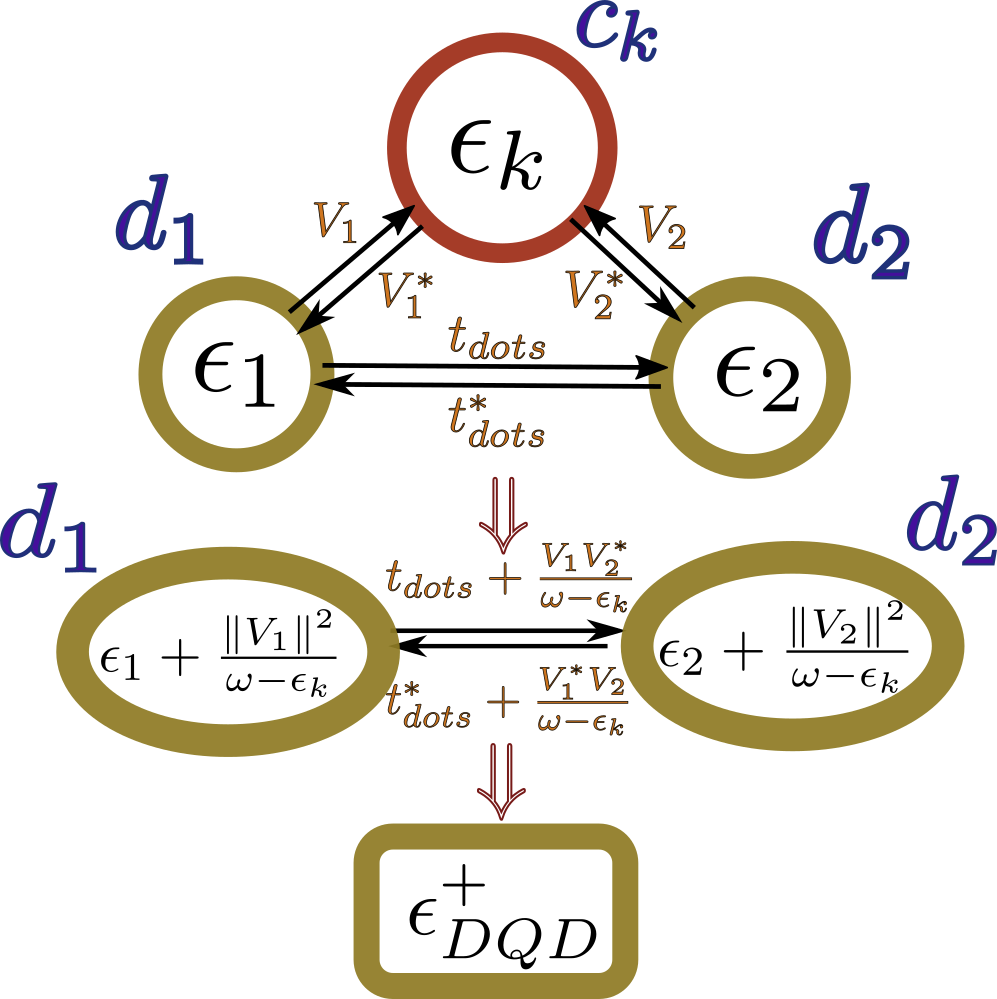
\includegraphics[scale=0.27]{Graficos/Graph_DQD-Pro.png}
        \caption{ 
        }
        %
        \label{fig:GraphsDQD}
        \end{center}
        \end{figure}
%-----------E N D  F I G U R E  1 ------




To explain the process of Gaussian elimination we will obtain the green function for the case without Majorana fermion $(t_1= t_2=0)$.  The transport matrix for this system is 
\begin{equation}
        \left[\begin{array}{ccc}
    \omega-\epsilon_{1} & -V_{1} & -t_{dots}\\
    -V_{1}^{*} & \omega-\epsilon_{k} & -V_{2}\\
    -t_{dots}^{*} & -V_{2}^{*} & \omega-\epsilon_{2}
    \end{array}\right]. \label{eq:DQDMatrix}
\end{equation}
\noindent The graph associated to this matrix can be observed in FIG\ref{fig:GraphsDQD}.a). To eliminate the vertex $c_k$ we just need to subtract from \eqref{eq:DQDMatrix} the rank-$1$ matrix that cancels the row and the column corresponding to $c_k$. This matrix is 
\begin{equation}
        \left[\begin{array}{ccc}
    \frac{V_{1}^{*}V_{1}}{\omega-\epsilon_{k}} & -V_{1}^{*} & \frac{V_{2}V_{1}^{*}}{\omega-\epsilon_{k}}\\
    -V_{1} & \omega-\epsilon_{k} & -V_{2}\\
    \frac{V_{2}^{*}V_{1}}{\omega-\epsilon_{k}} & -V_{2}^{*} & \frac{V_{2}^{*}V_{2}}{\omega-\epsilon_{k}}
    \end{array}\right]. \label{eq:rank1}
\end{equation}
The result of \eqref{eq:DQDMatrix} -  \eqref{eq:rank1} is 

\begin{equation}
        \left[\begin{array}{ccc}
    \omega-\epsilon_{1}-\frac{V_{1}^{*}V_{1}}{\omega-\epsilon_{k}} & 0 & -t_{dots}-\frac{V_{2}V_{1}^{*}}{\omega-\epsilon_{k}}\\
    0 & 0 & 0\\
    -t_{dots}^{*}-\frac{V_{2}^{*}V_{1}}{\omega-\epsilon_{k}} & 0 & \omega-\epsilon_{2}-\frac{V_{2}V_{1}^{*}}{\omega-\epsilon_{k}}
    \end{array}\right]
\end{equation}
\noindent which is depicted by the graphs in FIG.\ref{fig:GraphsDQD}.b). The next step is to pop-out the vertex $d_2$ following the same procedure. At the end, the energy inside the vertex $d_1$ will be
\begin{equation}
    \epsilon_{DQD}=\epsilon_{1}+\sum_{\mathbf{k}}\frac{V_{1}V_{1}^{*}}{\omega-\epsilon_{\mathbf{k}}}+\frac{\left\Vert t_{dots}+\sum_{\mathbf{k}}\frac{V_{1}V_{2}^{*}}{\omega-\epsilon_{\mathbf{k}}}\right\Vert ^{2}}{\omega-\epsilon_{2}-\sum_{\mathbf{k}}\frac{V_{2}V_{2}^{*}}{\omega-\epsilon_{\mathbf{k}}}} \label{eq:EnDQD}
\end{equation}
and the green function of $\Green{d_1d^\dagger_1}$ in a DQD will be given by $\frac{1}{\omega -  \epsilon_{DQD}}$ (see FIG.\ref{fig:GraphsDQD}.c)).

\subsection{Solution of the transport equations}

The previous procedure can be generalized into the following algorithm:

\begin{enumerate}
    \item To compute the transport equations with the second term fixed in the creation operator of the dot.
     \item To set up the  graph associated to the trasport system.
    \item To pop out the vertexes of the graph. Each pop-out proces carries the following steps.
    \begin{enumerate}
        \item To compute the extra-terms in the energies and couplings based on the walks passing through the vertex that will be popped out.
        \item To eliminate this vertex from the graph. 
        \item To iterate till there is just one  vertex.
        \end{enumerate}
    \item To invert the last energy to obtain the final green function of the dot.
\end{enumerate}

To solve  the general case we start with the graph in FIG.\ref{fig:Transport} and we pop out the vertexes $c_k,c^\dagger_k, d_{2,\dw}$ and $ d^\dagger_{2,\dw}$ in that order. The energies associated to $d_{1,\dw}$ and $d^\dagger_{1,\dw}$ will be similar to \eqref{eq:EnDQD} giving 
\begin{equation}
    \epsilon_{DQD}^{\pm}=\pm\epsilon_{1}+\sum_{\mathbf{k}}\frac{V_{1}V_{1}^{*}}{\omega-\epsilon_{\mathbf{k}}}+\frac{\left\Vert \pm t_{dots}+\sum_{\mathbf{k}}\frac{V_{1}V_{2}^{*}}{\omega-\epsilon_{\mathbf{k}}}\right\Vert ^{2}}{\omega\pm\epsilon_{2}-\sum_{\mathbf{k}}\frac{V_{2}V_{2}^{*}}{\omega-\epsilon_{\mathbf{k}}}}. \label{eq:epDQD}
\end{equation}
\noindent There is also a correction in the couplings between the Majorana mode and $d_{1,\dw}$, $d^\dagger_{1,\dw}$ given by 

\begin{equation}
    T_{\pm}=\pm t_{1}\pm t_{2}\frac{\left(\pm t_{dots}+\sum_{\mathbf{k}}\frac{V_{1}V_{2}^{*}}{\omega-\epsilon_{\mathbf{k}}}\right)}{\omega\pm\epsilon_{2}\pm\sum_{\mathbf{k}}\frac{V_{2}V_{2}^{*}}{\omega-\epsilon_{\mathbf{k}}}}. \label{eq:T+-}
\end{equation}

Finally since the Majorana is in contact with dot $2$, there is an extra-term appearing in the  Majorana energy given by 
\begin{equation}
    \epsilon_{M2}=\omega-\epsilon_{M}-\frac{\frac{\omega}{\omega+\epsilon_{M}}\left\Vert t_{2}\right\Vert ^{2} } {\omega-\epsilon_{2}-\sum_{\mathbf{k}}\frac{V_{2}V_{2}^{*}}{\omega-\epsilon_{\mathbf{k}}}}-\frac{\frac{\omega}{\omega+\epsilon_{M}}\left\Vert t_{2}\right\Vert ^{2}}{\omega+\epsilon_{2}-\sum_{\mathbf{k}}\frac{V_{2}V_{2}^{*}}{\omega+\epsilon_{\mathbf{k}}}}. \label{eq:M2}
\end{equation}
With all the terms of the graph in FIG.\ref{fig:Transport}.b) computed, it only remains to pop out vertexes $d^\dagger_1$ and $f_\dw$ in that order to obtain the green function in equation \eqref{eq:Green_NonInteracting}. 













%---------------------------------------------------------------------------
 



% %-----------F I G U R E  Graph ------
% \begin{figure}[bt]
% \begin{center}
% 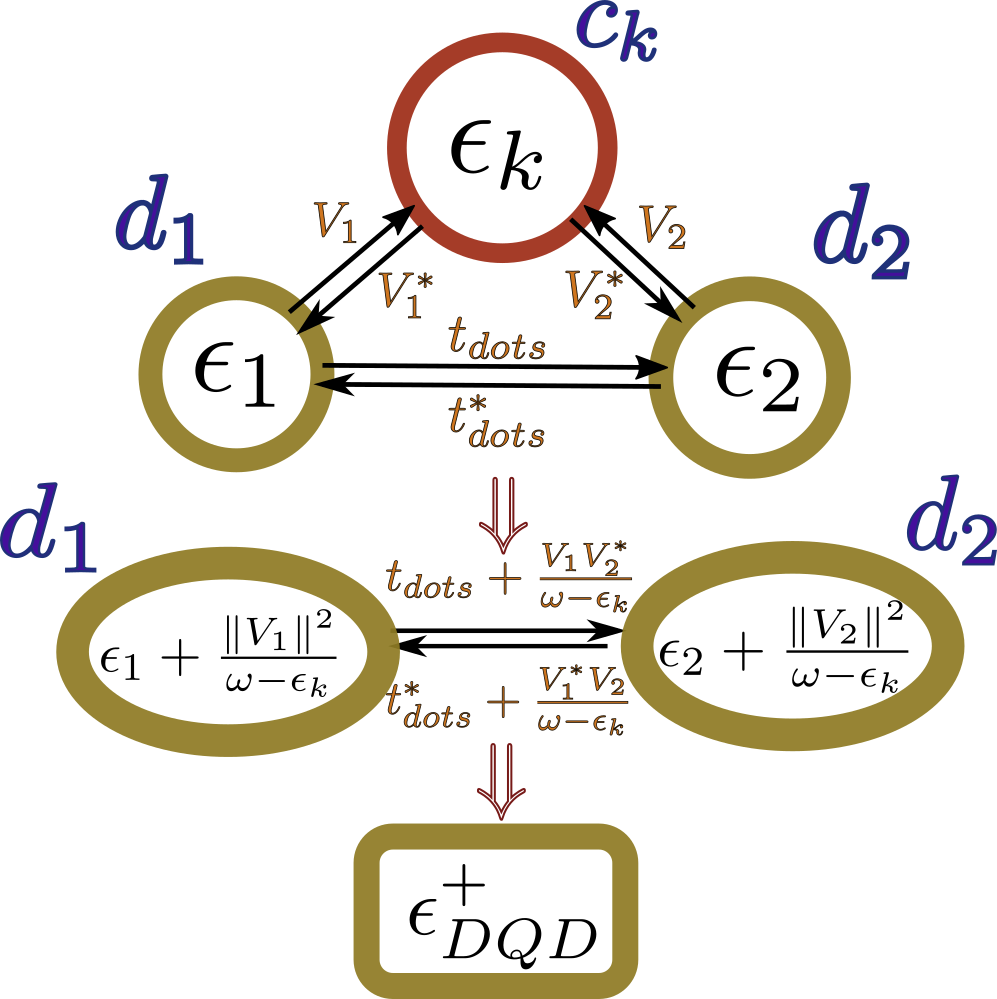
\includegraphics[scale=0.2]{Graficos/Graph_DQD-Pro.png}
% \caption{ 
% }
% %
% \label{fig:GenModel}
% \end{center}
% \end{figure}
% %-----------E N D  F I G U R E  1 ------





\end{document}



% \section{Atomic limit: Change of basis}
% Returning to Hamiltonian \eqref{eq:AtomicHam} the change of basis is given by 
% \[
%   d_{+ , \sigma} = \frac{1}{\sqrt{2}} (d_{1\sigma} +d_{2\sigma}) \ , \ 
%   d_{- , \sigma} = \frac{1}{\sqrt{2}} (d_{1\sigma} -d_{2\sigma}).
% \]

% These new operators satisfy the fermionic anti-commutation relations 
%  \[ \{d_{\pm , \sigma}, d^\dagger_{\pm , \sigma}\} = 1 , \{ d_{\pm , \sigma}, d^\dagger_{\mp , \sigma}\} = 0,
% \]
%  so that the may be considered as fermion operators. All lineal terms in \eqref{eq:AtomicHam} are trivially adapted to the new base. The repulsion potential 
% $$\sum_{i} (\sum_{\sigma} d_{i \sigma}^{\dagger}d_{i \sigma}-1)^{2} = (\sum_{\sigma} d_{1 \sigma}^{\dagger}d_{1 \sigma}-1)^{2} + (\sum_{\sigma} d_{2 \sigma}^{\dagger}d_{2 \sigma}-1)^{2} . $$ 
% gives rise to a non-trivial interaction between the new states. To find this interaction we define the particle number operator  
% \[\hat{n}_{i,\sigma}:= d^\dagger_{i,\sigma}d_{i,\sigma}.\] 

% So that 
% \begin{align}
% \hat{n}_{1,\sigma}= & \frac{1}{2} \left( \hat{n}_{+,\sigma} + \hat{n}_{-,\sigma} + d^\dagger_{+,\sigma}d_{-,\sigma} + d^\dagger_{-,\sigma}d_{+,\sigma} \right) \\
% = & \frac{1}{2} \left( \hat{N}_\sigma + \hat{E}_\sigma \right),
% \end{align}
% with $\hat{N}_\sigma = \hat{n}_{+,\sigma} + \hat{n}_{-,\sigma}$ and $\hat{E}_\sigma = d^\dagger_{+,\sigma}d_{-,\sigma} + d^\dagger_{-,\sigma}d_{+,\sigma}. $ Similarly 

% \[\hat{n}_{2,\sigma}= \frac{1}{2} \left( \hat{N}_\sigma - \hat{E}_\sigma \right).  \]
% Hence 
% \begin{align}
% \sum_{i} (\sum_{\sigma} d_{i \sigma}^{\dagger}d_{i \sigma}-1)^{2} = & \left(\frac{\hat{N} +\hat{E}}{2}-1 \right) ^{2} + \left( \frac{\hat{N} -\hat{E}}{2}-1 \right)^{2} \\
%  = & \frac{\left( \hat{N}-2 \right)^2- \hat{E}^2}{2},
% \end{align}

% with $\hat{N}_\sigma=\sum_\sigma \hat{N}_\sigma $ , $\hat{E}=\sum_\sigma \hat{E}_\sigma $. Note that opeator $\hat{N}$ represents the total occupation number inside both dots. If this occupation is different than $2$ there is an imbalance between particles and dots that is punished by this term. The term $E^2$ is much more interesting since this one is the responsible for the emergence of satellite peaks in the DOS. To understand what it makes it is simple to observe its results when applied to a based ordered by $\vert + , - \rangle$. 
% \[ \hat{E}^2 \vert \up , 0 \rangle =  \hat{E} \vert 0 , \up \rangle = \vert \up , 0 \rangle   \] 
% \[ \hat{E}^2 \vert \up , \dw \rangle =  \hat{E} \left( \vert 0 , \up\!\dw \rangle + \vert \up\!\dw , 0 \rangle \right) = 2\vert \up , \dw \rangle - 2\vert \dw , \up \rangle  \]

% \begin{align}
% H = \sum_{\sigma}  \frac{U}{4}\left( \left( \hat{N}-2 \right)^2- \hat{E}^2 \right) + \frac{t}{\sqrt{2}} (\gamma_1 d_{+,\dw}+d^\dagger_{+,\dw}\gamma_1 )
% \label{t+}
% \end{align}




 This system is already closed which means that we don't need any other equation to find the solution. The matrix form takes the form
 \begin{equation}
\left[\begin{array}{ccc}
\omega-\epsilon_{2} & -V_{2} & -t_{dots}\\
-V_{2}^{*} & \omega-\epsilon_{k} & -V_{1}\\
-t_{dots}^{*} & -V_{1}^{*} & \omega-\epsilon_{1}
\end{array}\right]\left[\begin{array}{c}
\Green{c_{\mathbf{k}},d_{1}^{\dagger}}\\
\Green{d_2,d_{1}^{\dagger}}\\
\Green{d_{1},d_{1}^{\dagger}}
\end{array}\right]=\left[\begin{array}{c}
0\\
0\\
1
\end{array}\right]
\label{eq:MatrixDQD}
 \end{equation}
 
\noindent By convenience we changed the order of the rows in the matrix. Although this matrix is not Laplacian, the procedure in \cite{spielman10} can still be applied with the downside of loosing some of the speed-up advantages of the algorithm. Still, some advantages of graphs are preserved. From these we point out  the possibility of taking taking minimal cuttings and the relation between these graphs and random walks in the graph. Both advantages simplify the complexity of the solution. 
 
Now, our objective is to compute the green function  $\Green{d_{1\downarrow},d_{1\downarrow}^{\dagger}}$.   For this we take the graph $\GDQD$ associated to the matrix in \eqref{eq:MatrixDQD}. The result is observed in \ref{fig:graphDQD}.a).  The vertexes of this graph will be the operators in the first site of the of the green functions  $(d_{1\downarrow},d_{2},c_{\boldsymbol{k}}$. $d_1^\dagger)$. $d^\dagger_1$ is not included since it only appears in the second sub-index of the green functions. The edges are given by the non-diagonal sites in the matrix. In addition, an energy parameter is assigned to each vertex, according to the corresponding term in the diagonal. These energies can also be taken as edges connecting each vertex with itself. 

% \begin{figure}[t]
%     \centering
%     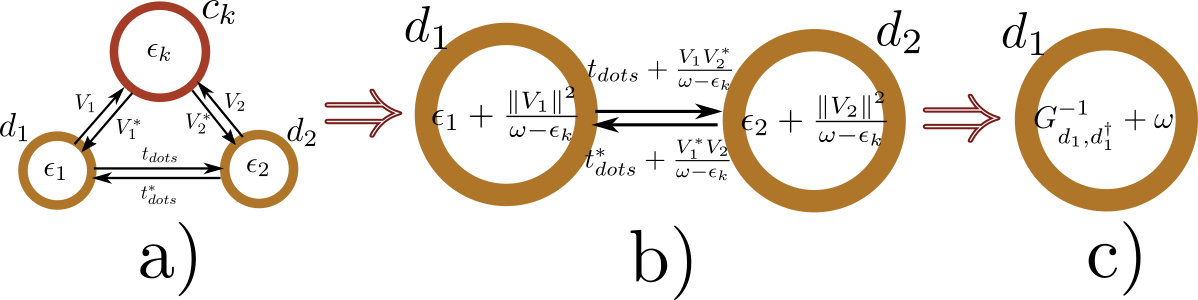
\includegraphics[scale=0.4]{IMAGES/Graphs/DQD-Pro.png}
%     \caption{ a) Graph $\GDQD$ b) After the elimination of vertex $c_k$, the energies of dots $d_1$ and $d_2$, and the coupling parameter are changed. c) After Gaussian elimination of dot $2$ the energy of dot $1$ is the inverse of $\Green{d_1,d^\dagger_1}$. \protect\Source{By the author.}}
%     \label{fig:graphDQD}
% \end{figure}


The algorithm consists in the following. Each step of Gauss-Jordan elimination leads to a new graph with different energies and couplings. The elimination of a row and column is equivalent to pop-out the corresponding vertex in the graph. For instance, lets eliminate the first row and column of the matrix in \eqref{eq:MatrixDQD}. For it we just need to subtract the rank-$1$ matrix with the same first row and first column. 
\begin{equation}
        \left[\begin{array}{ccc}
    \omega-\epsilon_{k} & -V_{2} & -V_{1}\\
    -V_{2}^{*} & \omega-\epsilon_{2} & -t_{dots}\\
    -V_{1}^{*} & -t_{dots}^{*} & \omega-\epsilon_{1}
    \end{array}\right]-\left[\begin{array}{ccc}
    \omega-\epsilon_{k} & -V_{2} & -V_{1}\\
    -V_{2}^{*} & \frac{V_{2}^{*}V_{2}}{\omega-\epsilon_{k}} & \frac{V_{2}^{*}V_{1}}{\omega-\epsilon_{k}}\\
    -V_{1}^{*} & \frac{V_{2}V_{1}^{*}}{\omega-\epsilon_{k}} & \frac{V_{1}^{*}V_{1}}{\omega-\epsilon_{k}}
    \end{array}\right]=\left[\begin{array}{ccc}
    0 & 0 & 0\\
    0 & \omega-\epsilon_{2}-\frac{V_{2}^{*}V_{2}}{\omega-\epsilon_{k}} & -t_{dots}-\frac{V_{2}^{*}V_{1}}{\omega-\epsilon_{k}}\\
    0 & -t_{dots}^{*}-\frac{V_{2}V_{1}^{*}}{\omega-\epsilon_{k}} & \omega-\epsilon_{1}-\frac{V_{1}^{*}V_{1}}{\omega-\epsilon_{k}}
    \end{array}\right]
    \label{eq:Gauss-Jordan} 
\end{equation}

The graph associated to this matrix can be observed in \ref{fig:graphDQD}.b). The first vertex corresponding to operator $c_k$ has been popped out. The energies and couplings are modified according to the possible walks passing through the vertex $c_k$.  For instance $d_1$'s energy $\epsilon_1$ receives an extra-term $\frac{V_{1}^{*}V_{1}}{\omega-\epsilon_{k}}$ representing an additional walk  from $d_1$ to $d_1$ passing through  $c_k$. The same logic can be applied to the other terms.  

The next  stage will turn out into a single vertex as in \ref{fig:graphDQD}.c). As a result of Gauss-Jordan elimination it turns out that the energy of this vertex is the inverse of the green function $G_{d_1d^\dagger_1}$. The final result is then 

\begin{equation}
    \Green{d_{1},d_{1}^{\dagger}}=\left[\left(\omega-\epsilon_{1}-\frac{V_{1}V_{1}^{*}}{\omega-\epsilon_{\mathbf{k}}}\right)-\frac{\left(t_{dots}+\frac{V_{1}V_{2}^{*}}{\omega-\epsilon_{\mathbf{k}}}\right)\left(t_{dots}+\frac{V_{1}V_{2}^{*}}{\omega-\epsilon_{\mathbf{k}}}\right)^{*}}{\omega-\epsilon_{2}-\frac{\Gamma_{2}^{2}}{\omega-\epsilon_{\mathbf{k}}}}\right]^{-1}. \label{eq:solGreen}
\end{equation}

Just one additional correction. Remember that every term including $\epsilon_k$ is summing over all possible energies in the momentum space. We avoided this sum during the process to avoid carrying this term during the process. But it is important to include it know.  

\begin{equation}
     \Green{d_{1},d_{1}^{\dagger}}=\left[\left(\omega-\epsilon_{1}-\sum_{\mathbf{k}}\frac{V_{1}V_{1}^{*}}{\omega-\epsilon_{\mathbf{k}}}\right)-\frac{\left(t_{dots}+\sum_{\mathbf{k}}\frac{V_{1}V_{2}^{*}}{\omega-\epsilon_{\mathbf{k}}}\right)\left(t_{dots}+\sum_{\mathbf{k}}\frac{V_{1}V_{2}^{*}}{\omega-\epsilon_{\mathbf{k}}}\right)^{*}}{\omega-\epsilon_{2}-\sum_{\mathbf{k}}\frac{\Gamma_{2}^{2}}{\omega-\epsilon_{\mathbf{k}}}}\right]^{-1}. \label{eq:SumSolGreen}
\end{equation}

\subsection{Graph Algorithm \label{sec:Algorithm}}

